% case name
\chapter{source}
%
% - Purpose & Description:
%     These first two parts give reader short details about the test case,
%     the physical phenomena involved, the geometry and specify how the numerical solution will be validated
%
\section{Purpose}
%
This test shows the capability of \telemac{3d} to manage multiple
sources of fluid and tracers.
It also demonstrates the ability to compute injection and conservation
of multiple tracers.
%
\section{Description}
%
We consider a basin at rest.
Sources are specified at some points of the mesh.
3 tracers are used, one is the sum of the 2 others.
%
% - Reference:
%     This part gives the reference solution we are comparing to and
%     explicits the analytical solution when available;
%
% bibliography can be here or at the end
%\subsection{Reference}
%
%
\subsection{Reference}
%

%
% - Geometry and Mesh:
%     This part describes the mesh used in the computation
%
%
\subsection{Geometry and Mesh}
%
\subsubsection{Bathymetry}
%
Flat bottom ($z$ = -1~m)\\
Constant water depth = 1~m
%
\subsubsection{Geometry}
%
Basin length = 100~m\\
Basin width = 40~m (figure \ref{t3d:source:mesh_vel})
%
\subsubsection{Mesh}
%
674 triangular elements\\
373 nodes\\
5 layers regularly spaced on the vertical
%
% - Physical parameters:
%     This part specifies the physical parameters
%
%
\subsection{Physical parameters}
%
Constant vertical and horizontal viscosities: 10$^{-6}$ m$^2$/s\\
Coriolis: no\\
Wind: no
%
% Experimental results (if needed)
%\subsection{Experimental results}
%
% bibliography can be here or at the end
%\subsection{Reference}
%
% Section for computational options
%\section{Computational options}
%
% - Initial and boundary conditions:
%     This part details both initial and boundary conditions used to simulate the case
%
%
\subsection{Initial and Boundary Conditions}
%
\subsubsection{Initial conditions}
%
No velocity\\
Null water level\\
No tracers
%
\subsubsection{Boundary conditions}
%
Channel banks: solid boundary without roughness\\
Bottom: solid boundary roughness
%
\subsection{General parameters}
%
Time step: 1.1~s\\
Simulation duration: 1,100~s
%
% - Numerical parameters:
%     This part is used to specify the numerical parameters used
%     (adaptive time step, mass-lumping when necessary...)
%
%
\subsection{Numerical parameters}
%
Hydrostatic simulation\\
Advection of velocities: characteristics\\
Advection of tracers: edge by edge explicit finite volume Leo Postma
scheme for tidal flats
%
\subsection{Definition of sources}
%
Position source 1: $x \approx$ -21.6~m, $y \approx$ 5.3~m, $z$ = -0.5~m\\
Position source 2: $x \approx$ -0.8~m, $y \approx$ -10.~m, $z$ = -0.5~m\\
Constant discharge of 1~m$^3$/s at both sources\\
Tracer concentration at sources: 10~g/L (or kg/m$^3$)\\
Source 1 discharges tracer 1 and 2\\
Source 2 discharges tracer 2 and 3\\
Source 2 has an initial velocity: $U$ = 0.5~m/s, $V$ = 2~m/s\\
%
The definition of the discharges and tracer concentrations at sources
has been done in the \telkey{SOURCES FILE}.
As this last file is present in the examples directory, the keyword
\telkey{VALUES OF THE TRACERS AT THE SOURCES} is ignored but is given
as an example coherent with what is done in the \telkey{SOURCES FILE}.
%
\subsection{Comments}
%
% - Results:
%     We comment in this part the numerical results against the reference ones,
%     giving understanding keys and making assumptions when necessary.
%
%
\section{Results}
%
Figure \ref{t3d:source:mesh_vel} shows the horizontal mesh and sources
positions in the upper panel.

\begin{figure} [H]
\centering
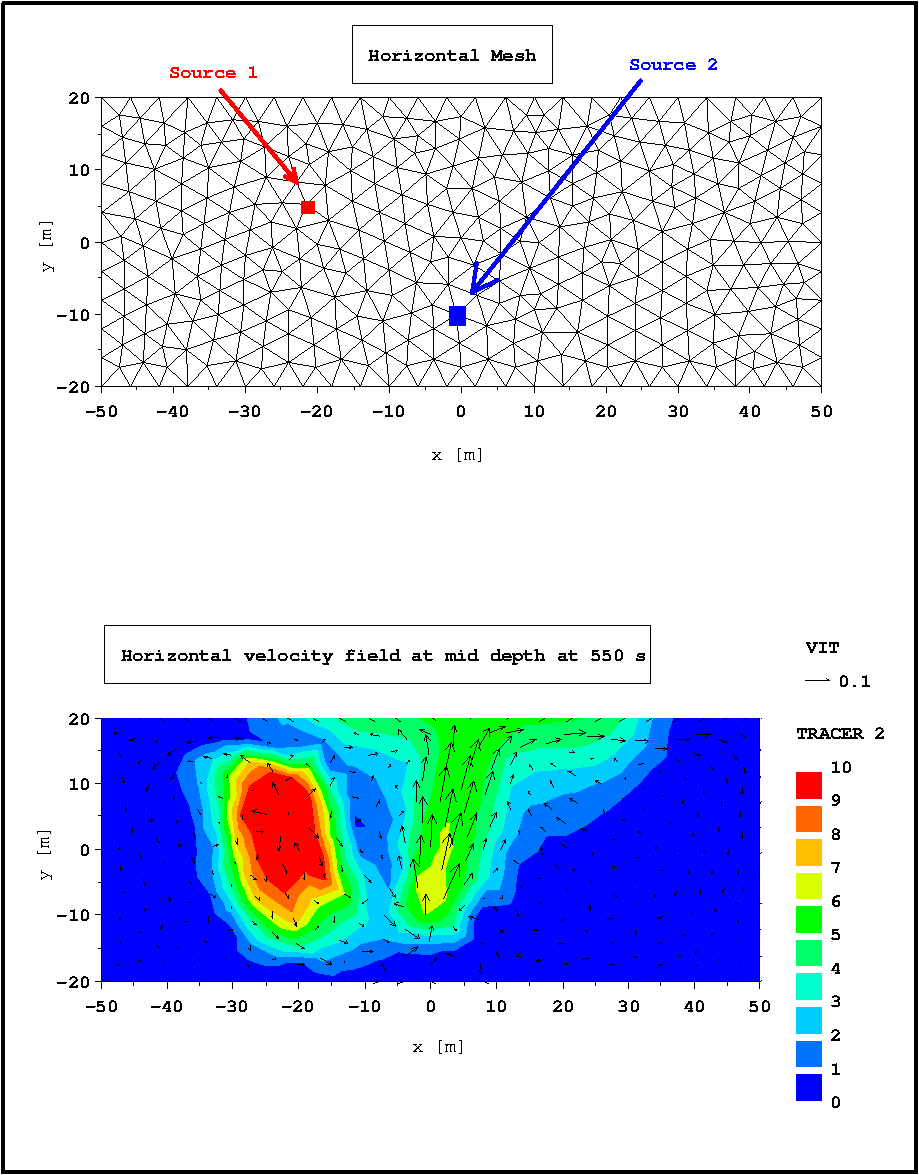
\includegraphics[scale=1.]{../img/source_mesh_vit.pdf}
 \caption{Source test: Mesh and horizontal velocity field}
 \label{t3d:source:mesh_vel}
\end{figure}

The lower panel highlights the influence of the initial velocity of
source 2 on the horizontal velocity field at mid depth at 550~s.
Additionally, the lower panel shows tracer 2 spreads in every direction
at source 1, unlike at source 2 where tracer 2 diffuses in the initial
velocity direction.

The horizontal and vertical plumes of each tracer at 1,100~s, on
figures \ref{t3d:source:hor_shape} and \ref{t3d:source:ver_shape}
respectively, allows verifying that the plume of tracer 2 is the
combination of the plumes of tracer 1 and 3.

\begin{figure} [H]
\centering
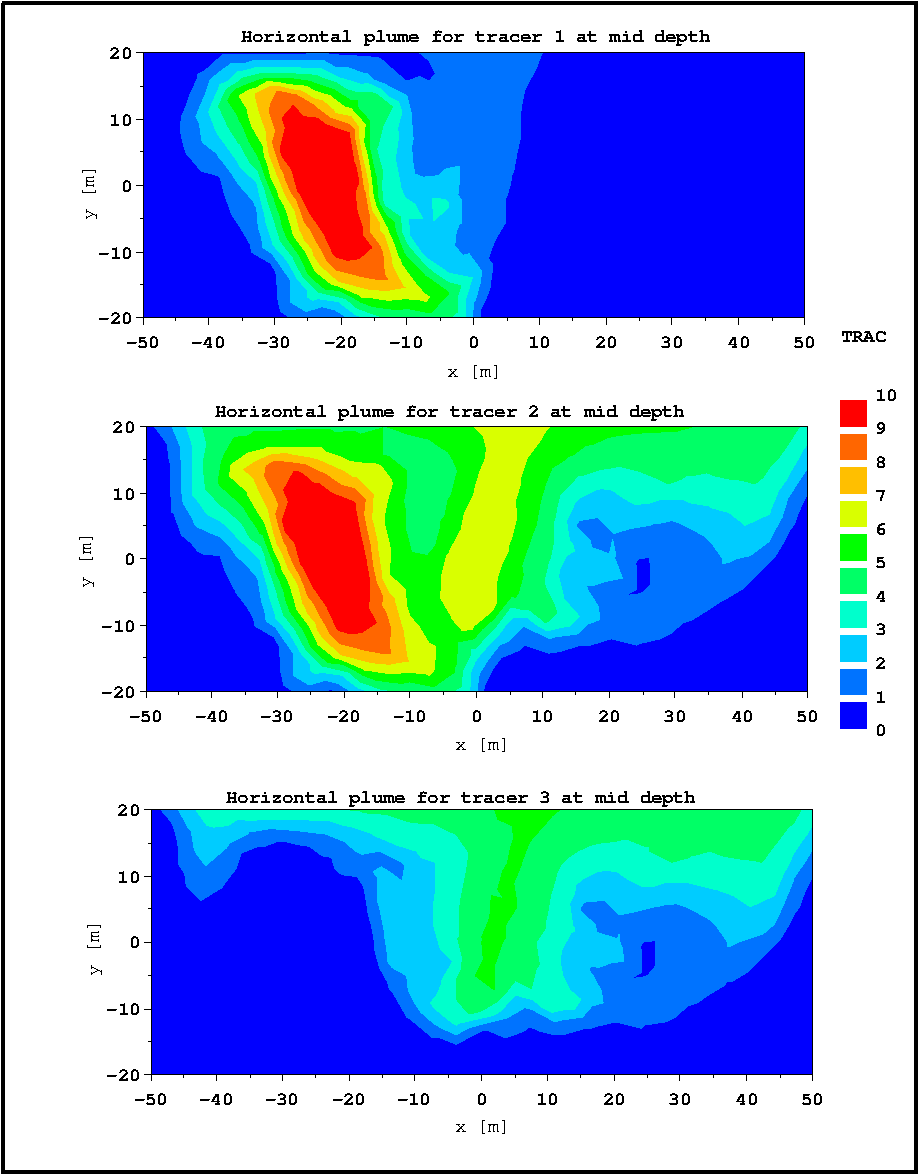
\includegraphics[scale=1.]{../img/source_hor_shape.pdf}
 \caption{Source test: Horizontal shape of the plumes}
 \label{t3d:source:hor_shape}
\end{figure}

\begin{figure} [H]
\centering
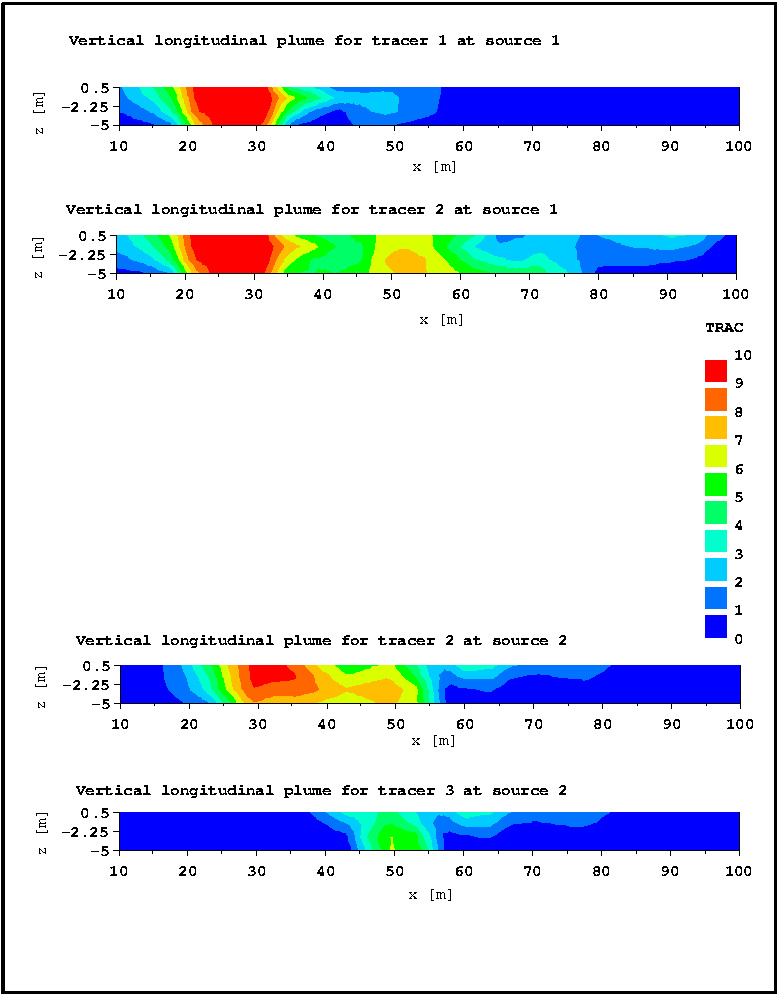
\includegraphics[scale=1.]{../img/source_ver_shape.pdf}
 \caption{Source test: Vertical shape of the plumes}
 \label{t3d:source:ver_shape}
\end{figure}

Moreover, the following mass balance of the \telemac{3d} simulation
shows that the amount of water injected by the sources is very good
(2,200~m$^3$ = 2 sources $\times$ 1~m$^3$/s $\times$ 1,100~s
with an error lower than 10$^{-6}~\rm{m}^3$, thus a relative error
lower than 10$^{-9}$).
If the keywords for accuracy for propagation and diffusion of tracers
are equal to 10$^{-14}$, the error becomes lower than
$10^{-12}~\rm{m}^3$, thus a relative error lower than the machine
accuracy 10$^{-15}$).
The mass balance also shows the conservation and the amount of
discharged tracer 1, 2 and 3 is good
(e.g. for tracer 2: 10~kg/m$^3 \times$ 2 sources $\times$ 1,100~s
$\times$ 1~m$^3$/s = 22,000~kg with an error lower than 10$^{-5}$~kg,
so a relative error lower than 10$^{-9}$).
To get an error lower than 2.10$^{-8}$~kg, so a relative error lower
than 2.10$^{-12}$, an accuracy of 10$^{-14}$ is required for the
diffusion of tracers and propagation.
Otherwise, the mass balances may be worse but sufficient enough,
depending on the accuracy the user wishes.

Balance for \telkey{ACCURACY FOR PROPAGATION} $= 10^{-8}$ and
\telkey{ACCURACY FOR DIFFUSION OF TRACERS} $= 10^{-9}$ in serial:
%
\begin{lstlisting}[language=TelFortran]
                        FINAL MASS BALANCE
        T =        1100.0000

        --- WATER ---
        INITIAL MASS                        :     4000.000
        FINAL MASS                          :     6200.000
        MASS LEAVING THE DOMAIN (OR SOURCE) :    -2200.000
        MASS LOSS                           :    0.2391803E-06

        --- TRACER 1: TRACER 1        , UNIT : ??              * M3)
        INITIAL MASS                        :     0.000000
        FINAL MASS                          :     11000.00
        MASS EXITING (BOUNDARIES OR SOURCE) :    -11000.00
        MASS LOSS                           :    0.5897147E-05

        --- TRACER 2: TRACER 2        , UNIT : ??              * M3)
        INITIAL MASS                        :     0.000000
        FINAL MASS                          :     22000.00
        MASS EXITING (BOUNDARIES OR SOURCE) :    -22000.00
        MASS LOSS                           :    0.2584195E-05

        --- TRACER 3: TRACER 3        , UNIT : ??              * M3)
        INITIAL MASS                        :     0.000000
        FINAL MASS                          :     11000.00
        MASS EXITING (BOUNDARIES OR SOURCE) :    -11000.00
        MASS LOSS                           :   -0.3261903E-05
\end{lstlisting}

Balance for \telkey{ACCURACY FOR PROPAGATION} $= 10^{-8}$ and
\telkey{ACCURACY FOR DIFFUSION OF TRACERS} $= 10^{-9}$ in parallel
(4 processors):
%
\begin{lstlisting}[language=TelFortran]
                        FINAL MASS BALANCE
        T =        1100.0000

        --- WATER ---
        INITIAL MASS                        :     4000.000
        FINAL MASS                          :     6200.000
        MASS LEAVING THE DOMAIN (OR SOURCE) :    -2200.000
        MASS LOSS                           :    0.2392089E-06

        --- TRACER 1: TRACER 1        , UNIT : ??              * M3)
        INITIAL MASS                        :     0.000000
        FINAL MASS                          :     11000.00
        MASS EXITING (BOUNDARIES OR SOURCE) :    -11000.00
        MASS LOSS                           :    0.5897227E-05

        --- TRACER 2: TRACER 2        , UNIT : ??              * M3)
        INITIAL MASS                        :     0.000000
        FINAL MASS                          :     22000.00
        MASS EXITING (BOUNDARIES OR SOURCE) :    -22000.00
        MASS LOSS                           :    0.2584398E-05

        --- TRACER 3: TRACER 3        , UNIT : ??              * M3)
        INITIAL MASS                        :     0.000000
        FINAL MASS                          :     11000.00
        MASS EXITING (BOUNDARIES OR SOURCE) :    -11000.00
        MASS LOSS                           :   -0.3261772E-05
\end{lstlisting}

Balance for \telkey{ACCURACY FOR PROPAGATION} $= 10^{-14}$ and
\telkey{ACCURACY FOR DIFFUSION OF TRACERS} $= 10^{-14}$ in serial:
%
\begin{lstlisting}[language=TelFortran]
                        FINAL MASS BALANCE
        T =        1100.0000

        --- WATER ---
        INITIAL MASS                        :     4000.000
        FINAL MASS                          :     6200.000
        MASS LEAVING THE DOMAIN (OR SOURCE) :    -2200.000
        MASS LOSS                           :    0.4547474E-12

        --- TRACER 1: TRACER 1        , UNIT : ??              * M3)
        INITIAL MASS                        :     0.000000
        FINAL MASS                          :     11000.00
        MASS EXITING (BOUNDARIES OR SOURCE) :    -11000.00
        MASS LOSS                           :   -0.1768058E-07

        --- TRACER 2: TRACER 2        , UNIT : ??              * M3)
        INITIAL MASS                        :     0.000000
        FINAL MASS                          :     22000.00
        MASS EXITING (BOUNDARIES OR SOURCE) :    -22000.00
        MASS LOSS                           :   -0.1020817E-07

        --- TRACER 3: TRACER 3        , UNIT : ??              * M3)
        INITIAL MASS                        :     0.000000
        FINAL MASS                          :     11000.00
        MASS EXITING (BOUNDARIES OR SOURCE) :    -11000.00
        MASS LOSS                           :    0.7525159E-08
\end{lstlisting}
%
\section{Conclusion}
%
\telemac{3d} is able to compute the evolution and conservation of
tracers discharged by sources.
%
% Here is an example of how to include the graph generated by validateTELEMAC.py
% They should be in test_case/img
%\begin{figure} [!h]
%\centering
%\includegraphics[scale=0.3]{../img/mygraph.png}
% \caption{mycaption}\label{mylabel}
%\end{figure}
%
% bibliography
%\section{Reference}
